% iaus2esa.tex -- sample pages for Proceedings IAU Symposium document class
% (based on v1.0 cca2esam.tex)
% v1.04 released 17 May 2004 by TechBooks
%% small changes and additions made by KAvdH/IAU 4 June 2004
% Copyright (2004) International Astronomical Union

\NeedsTeXFormat{LaTeX2e}

\documentclass{iaus}
\usepackage{graphicx}

\newcommand{\unit}[2]{\ensuremath{\textrm{#1}^{#2}}}
\newcommand{\sub}[2]{\ensuremath{#1_{\mathrm{#2}}}}
\newcommand{\half}{\frac{1}{2}}


\title[Galactic potential from tidal stream actions] %% give here short title %%
{Action-space clustering of tidal streams to map the Galactic potential}

\author[R.E. Sanderson, A. Helmi, \& D. Hogg]   %% give here short author list %%
{Robyn E. Sanderson$^1$, Amina Helmi $^1$,
%%  \thanks{Present address: Fluid Mech Inc., 24 The Street, Lagos, Nigeria.},
 \and David Hogg$^2$}

\affiliation{$^1$ Kapteyn Astronomical Institute, P.O. Box 800, 9700AV Groningen, Netherlands\\ email: {\tt sanderson@astro.rug.nl} \\[\affilskip]
$^2$ Center for Cosmology and Particle Physics, Department of Physics, New York University, 4 Washington Place, New York, NY  10003, USA}

\pubyear{2014}
\volume{298}  %% insert here IAU Symposium No.
\pagerange{XX -- YY}
% \date{?? and in revised form ??}
\setcounter{page}{1}
\jname{IAUS\,298 Setting the scene for Gaia and LAMOST}
\editors{S. Feltzing, G. Zhao, N.\,A. Walton \& P.\,A. Whitelock, eds.}
\begin{document}

\maketitle

\begin{abstract}
Given a parameterized model of the Galactic potential, the best-fit parameters can be obtained by maximizing the Kullback-Leibler divergence of the action distribution of a set of stars initially clustered in action space (e.g. stars in tidal streams). This method will allow us to map the Milky Way�s gravitational potential by simultaneously fitting multiple tidal streams without requiring stream membership information. With 20 streams of at least 20 stars each, including observational errors consistent with predictions for Gaia, this technique recovers the input potential parameters to a precision of $\pm$0.1 dex and an accuracy of 0.05 dex. With all the observed streams in our mock stellar halo (about 40) that fit the error criteria, the precision improves to $\pm$0.05 dex.

\keywords{Galaxy: structure, Galaxy: halo, Galaxy: kinematics and dynamics, stars: kinematics, methods: data analysis, methods: statistical, surveys}
%% add here a maximum of 10 keywords, to be taken form the file <Keywords.txt>
\end{abstract}

\firstsection % if your document starts with a section,
              % remove some space above using this command.
\section{Introduction}
Gaia will measure the complete six-dimensional phase space positions of an unprecedentedly large set of Galactic halo stars. This will allow us to search for and study tidal streams in  spaces other than the standard positions and velocities $(\mathbf{x}, \mathbf{v})$. One particularly useful space is that of the angles and actions $(\mathbf{\theta}, \mathbf{J})$. In this space, for a time-independent or adiabatically varying potential, the evolution of streams with time is quite simple: the angles $\mathbf{\theta}$ evolve linearly with time and the actions $\mathbf{J}$ are adiabatically invariant. Furthermore for a tidal stream created by the disruption of a satellite galaxy or globular cluster, the small initial phase-space volume of such a system implies that the actions of the stream stars will be tightly clustered in action space. This property of stream star actions can be used to constrain the potential because the actions depend on the gravitational potential: the clustering is tightest for actions computed using the best-fit potential. 

%\begin{figure}
%\begin{center}
%\begin{tabular}{ccc}
% 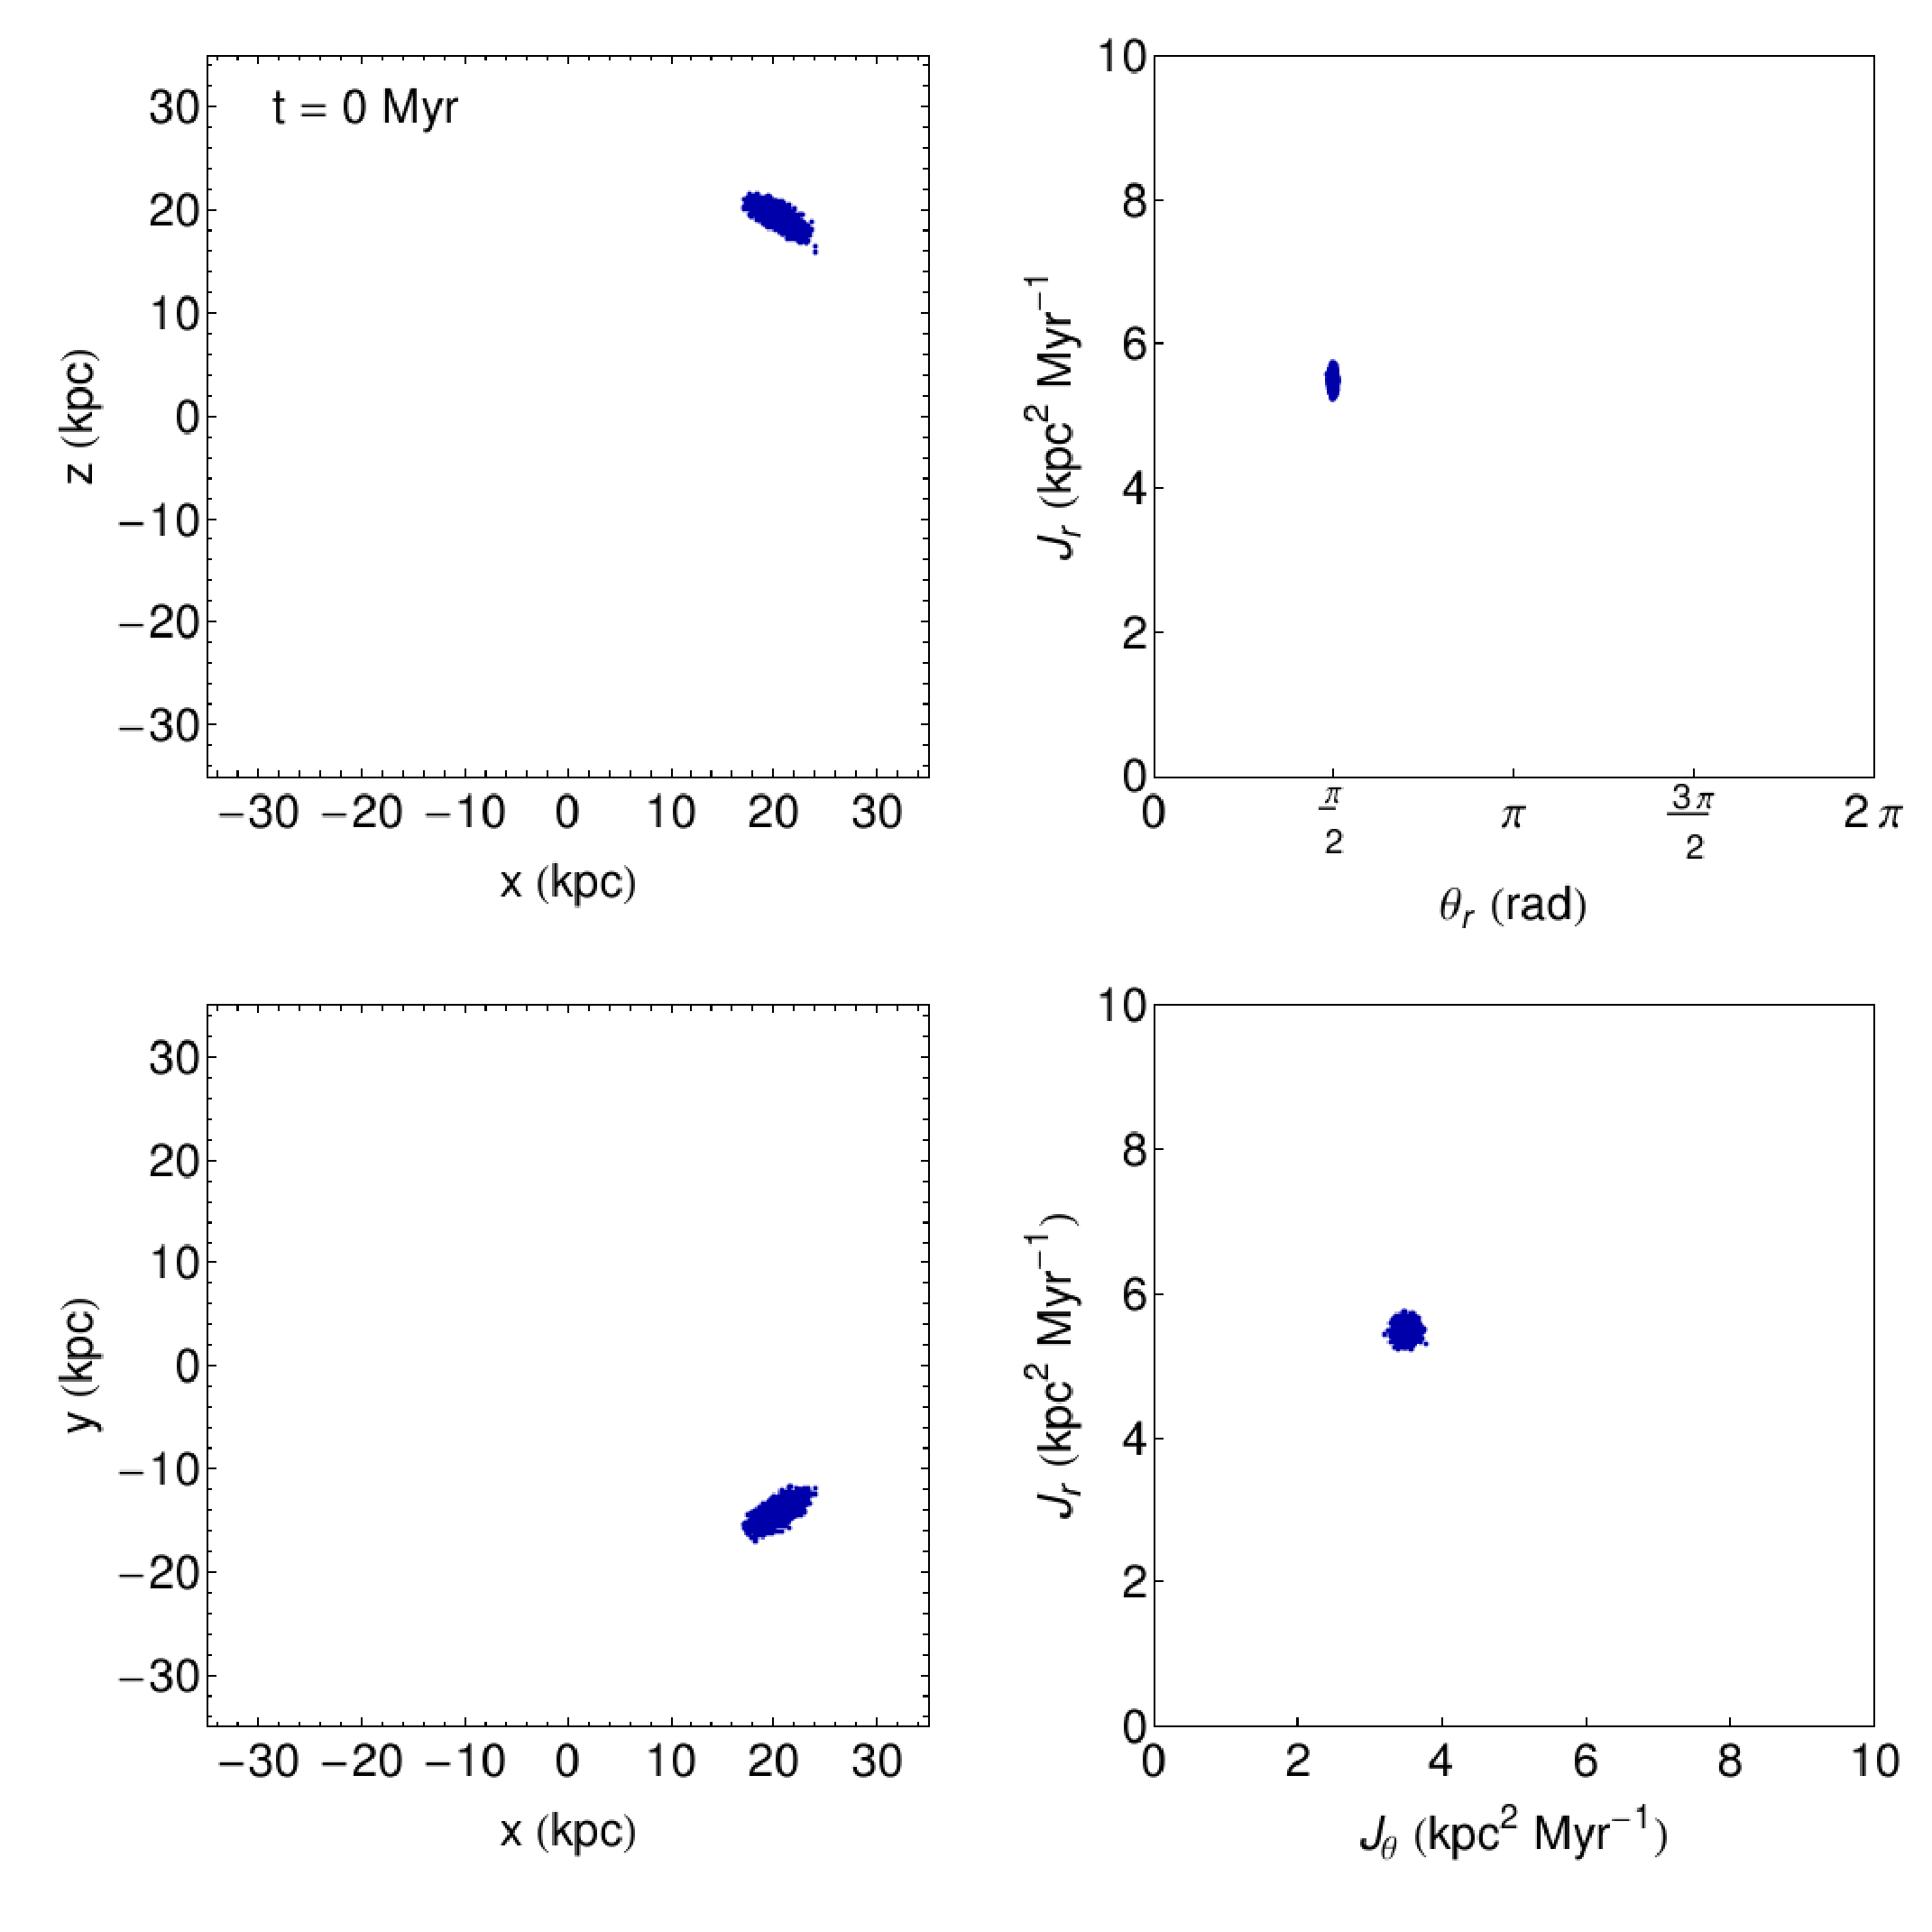
\includegraphics[width=1.6in]{Sanderson_Robyn_fig1_a.ps}  &
% 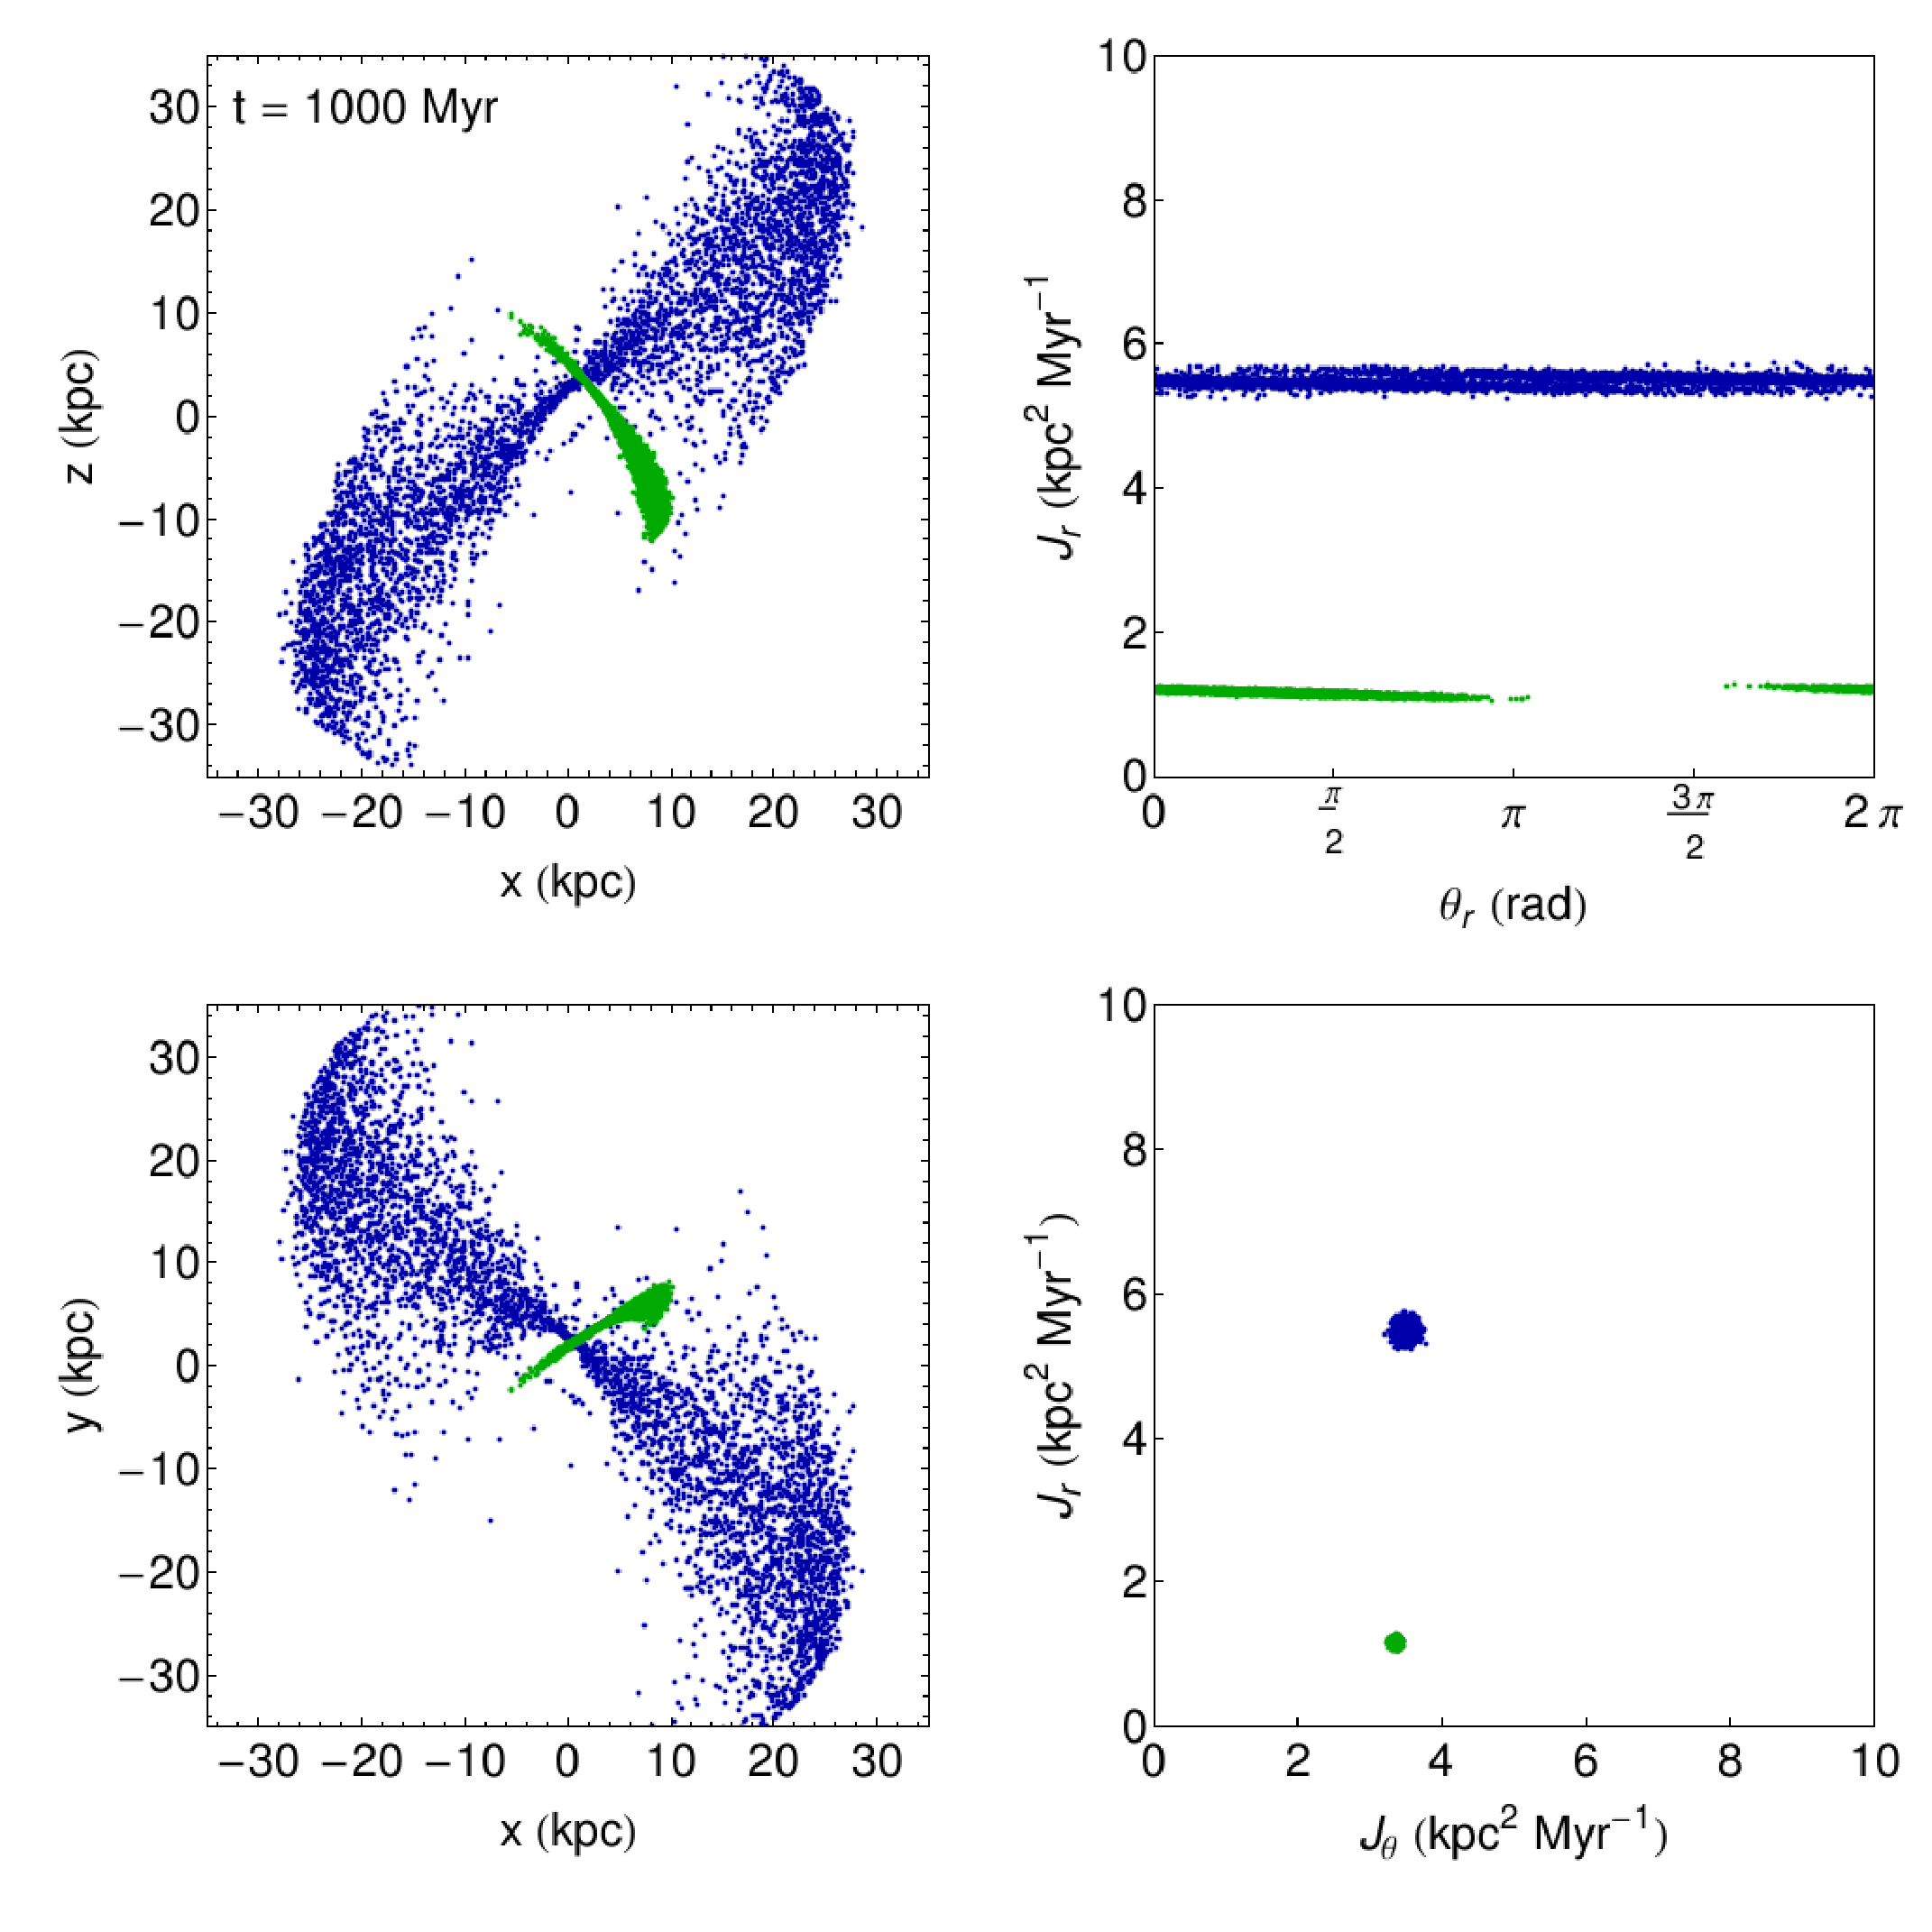
\includegraphics[width=1.6in]{Sanderson_Robyn_fig1_b.ps}  & 
%  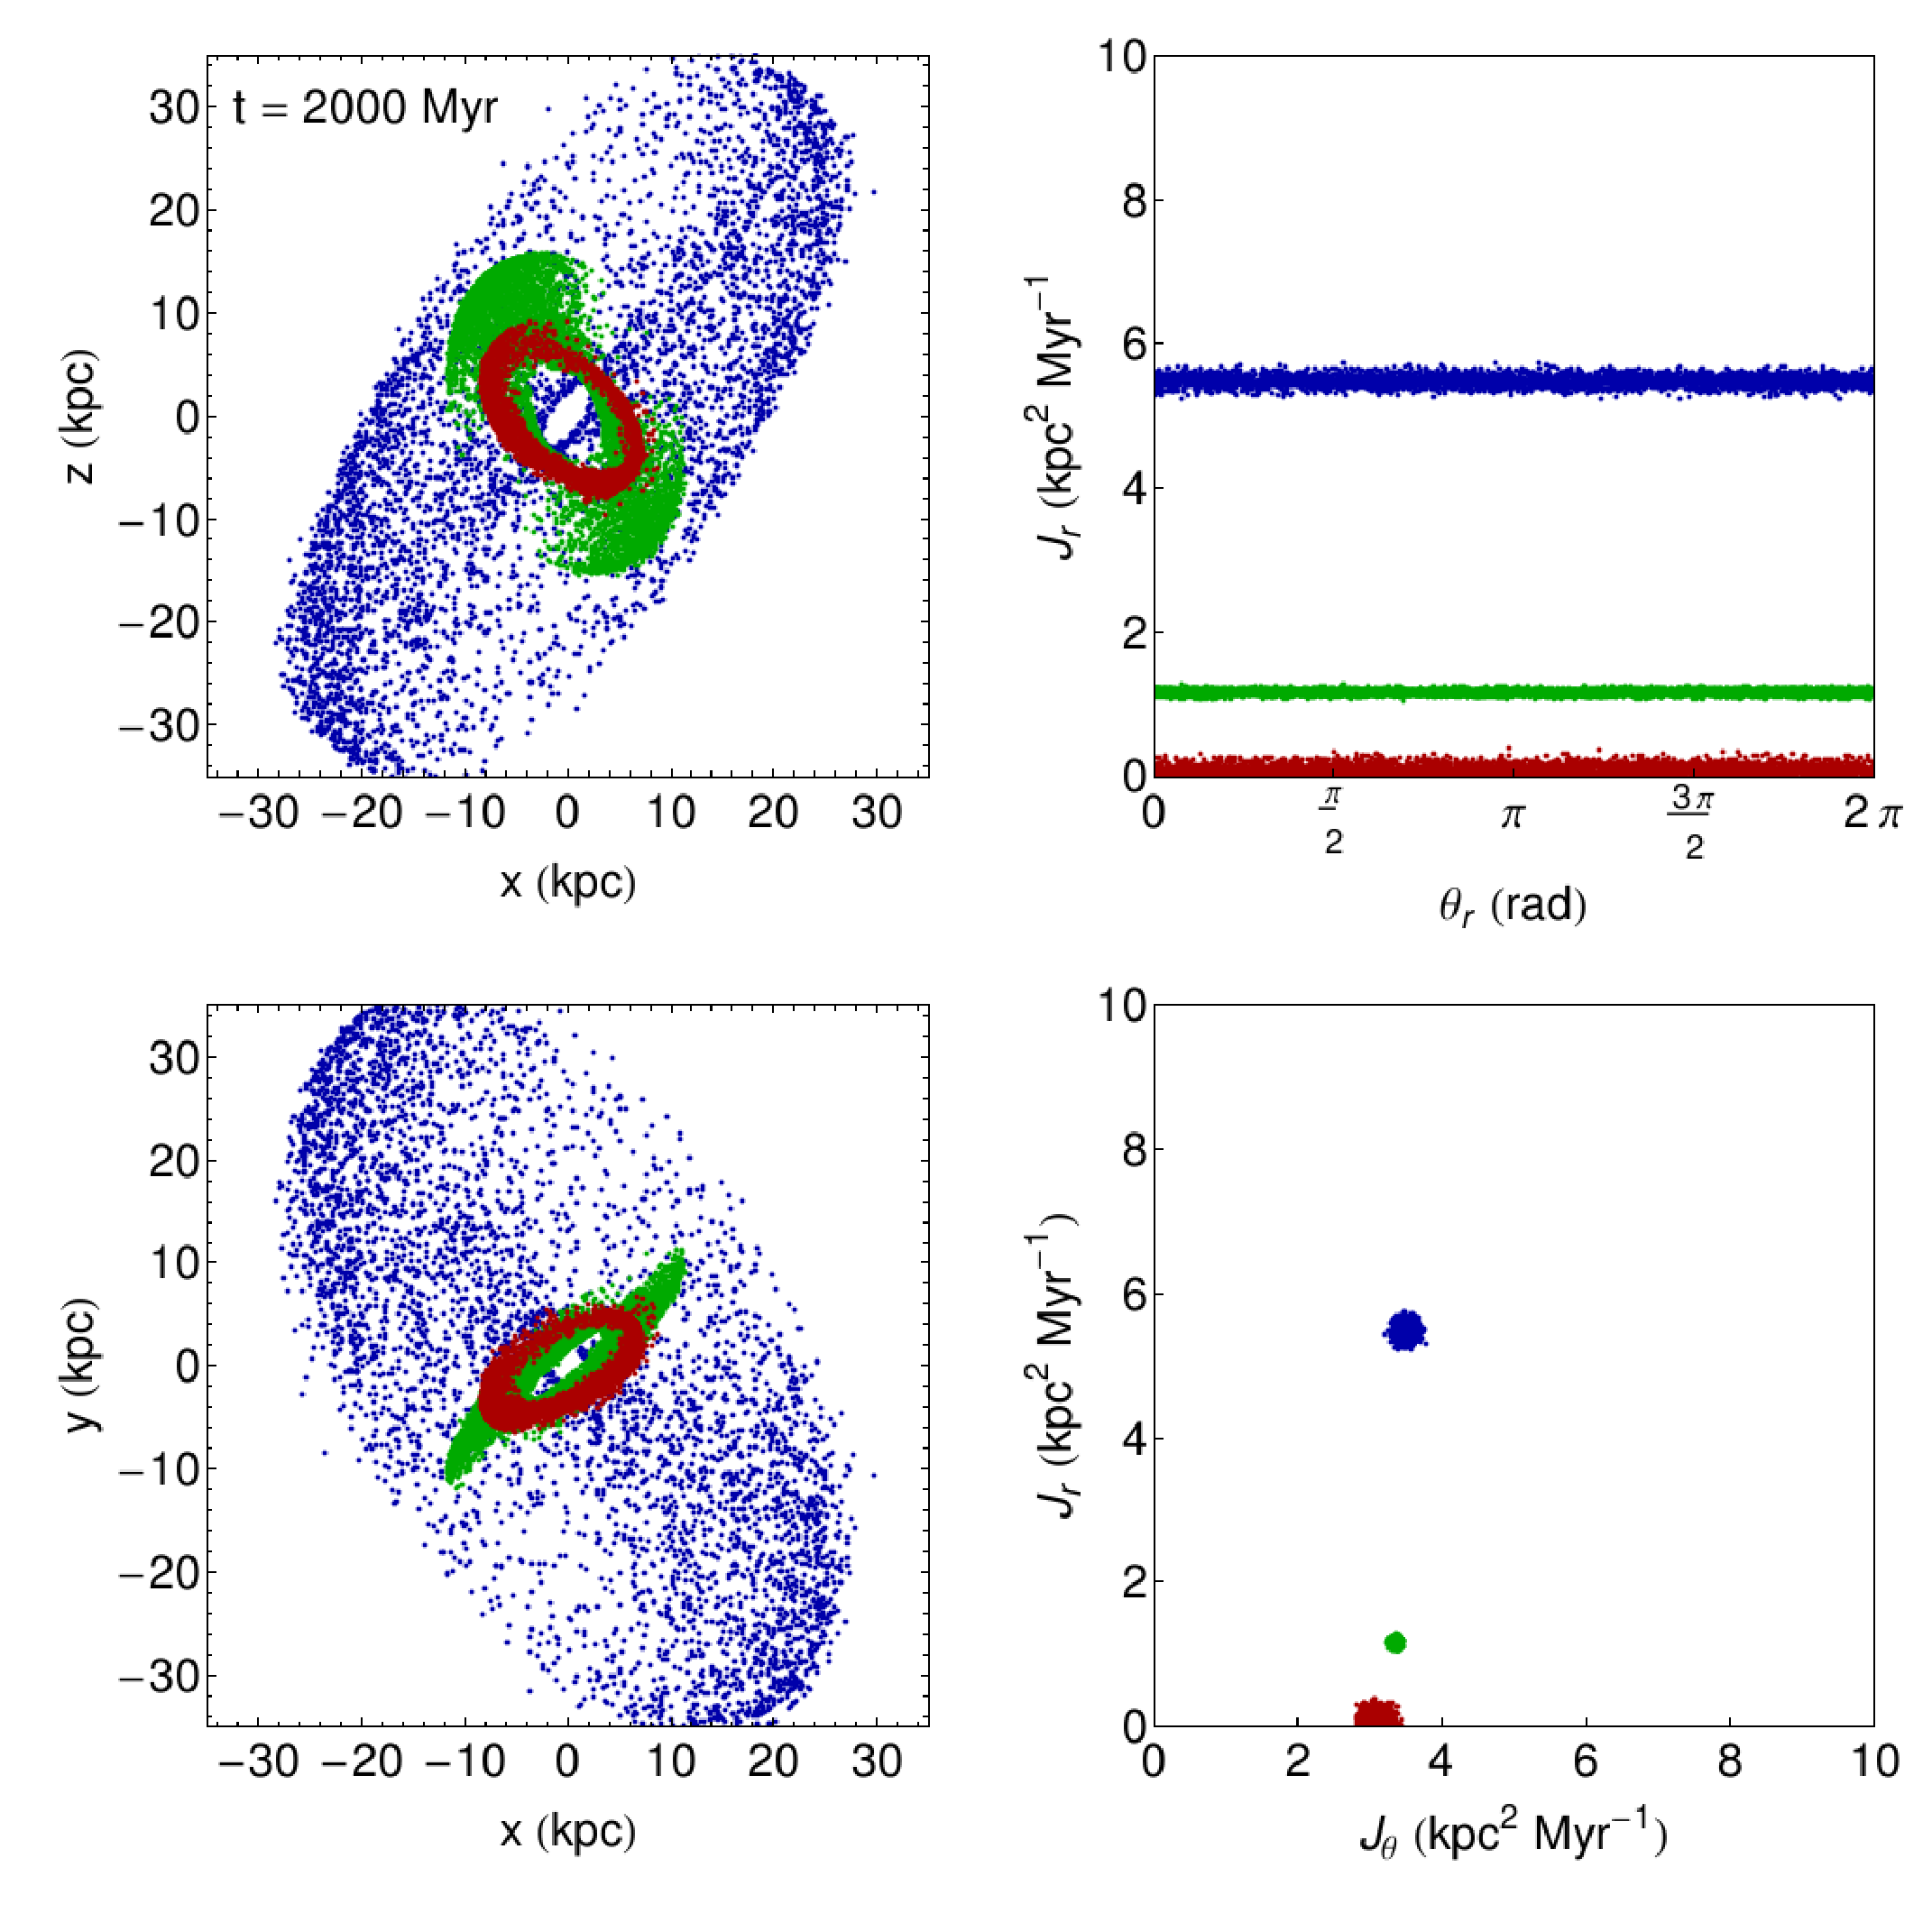
\includegraphics[width=1.6in]{Sanderson_Robyn_fig1_c.ps} 
%\end{tabular} 
% % Plesae ensure all files are named according to instructions (see instructions to authors).
% \caption{Views of three tidal streams of different ages on different orbits in a static isochrone potential, shown at three different times: infall of the oldest stream (left), just after infall of the next-oldest stream (center), and after all three streams have evolved over many orbits (right). Over time the position distribution (left column) becomes complex and the angles (top right) become phase-mixed, but the action distribution (bottom right) remains clustered.  }
%   \label{RES:fig1} % please use unique labels, such as your initials NNN:fig1
%\end{center}
%\end{figure}

We use the Kullback-Leibler divergence \cite[KLD; Kullback \& Leibler 1951]{Kullback1951}, which measures clustering, as a merit function to find the best-fit gravitational potential. For a continuous random variable $\mathbf{x}$, the KLD \emph{from} distribution $p(\mathbf{x})$ (e.g. the action distribution of the stream stars) \emph{to} a comparison distribution $q(\mathbf{x})$ is defined as
\begin{equation}
 D_{KL}(p || q) \equiv \int p(\mathbf{x}) \log \frac{p(\mathbf{x})}{q(\mathbf{x})} d\mathbf{x}.
\end{equation}
The KLD is not symmetric; it can be considered a measure of the relative entropy between $p$ and $q$. The lower the entropy (i.e., the higher the clustering) of $p$ relative to $q$, the higher the value of $D_{KL}$.
%
%\begin{figure}
%\begin{center}
%\begin{tabular}{cc}
% 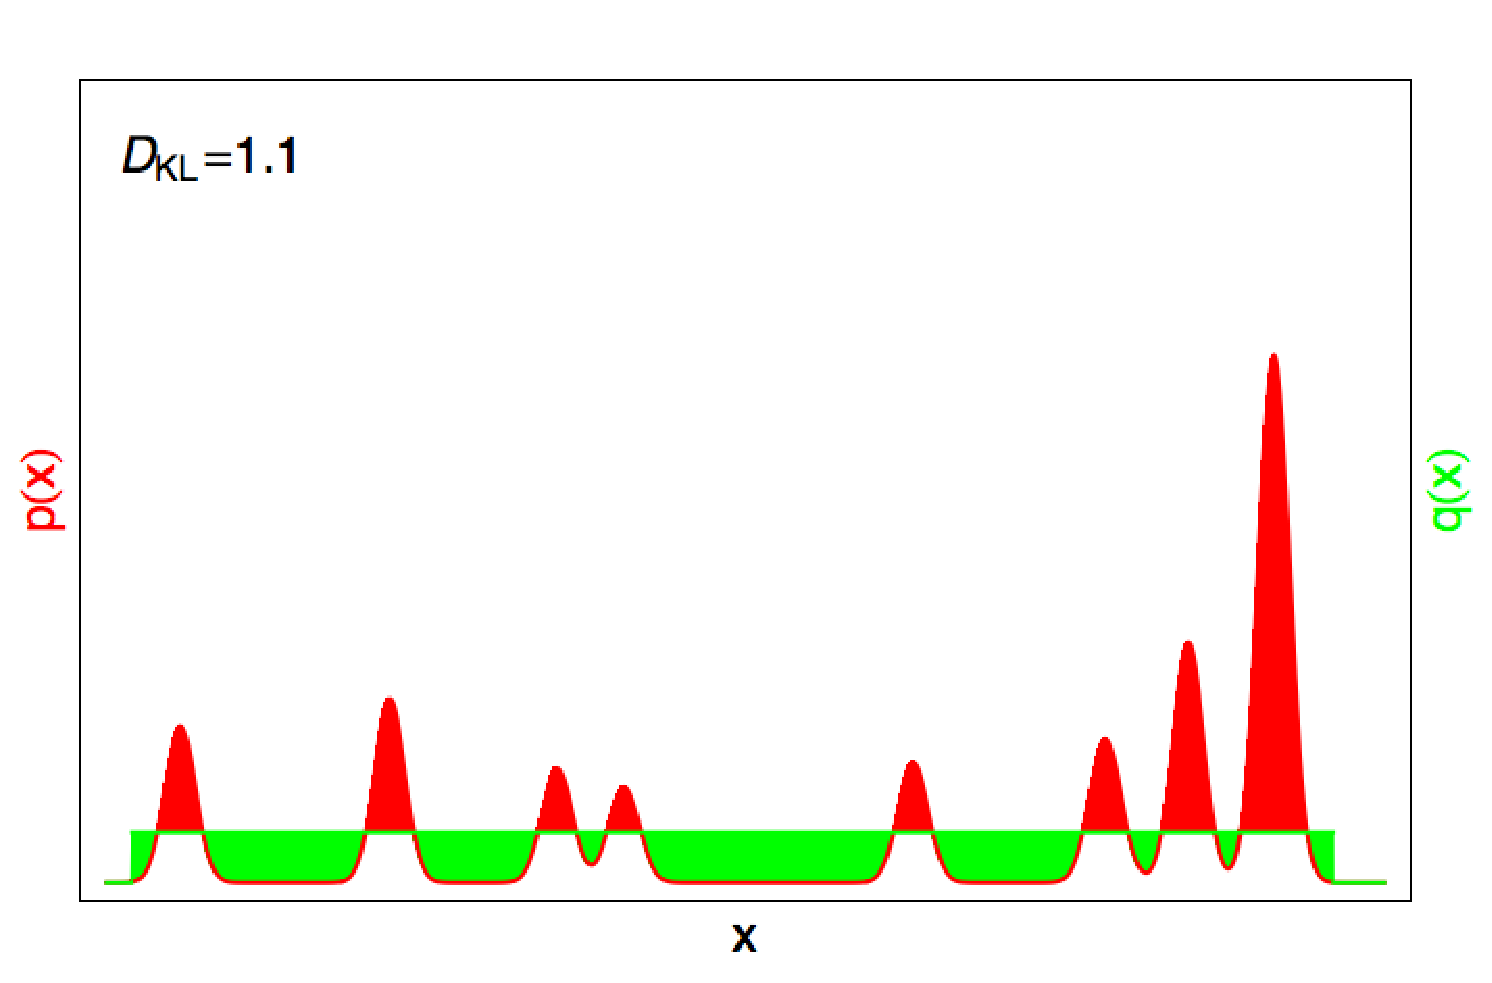
\includegraphics[width=2.4in]{Sanderson_Robyn_fig2_a.eps}  &
% 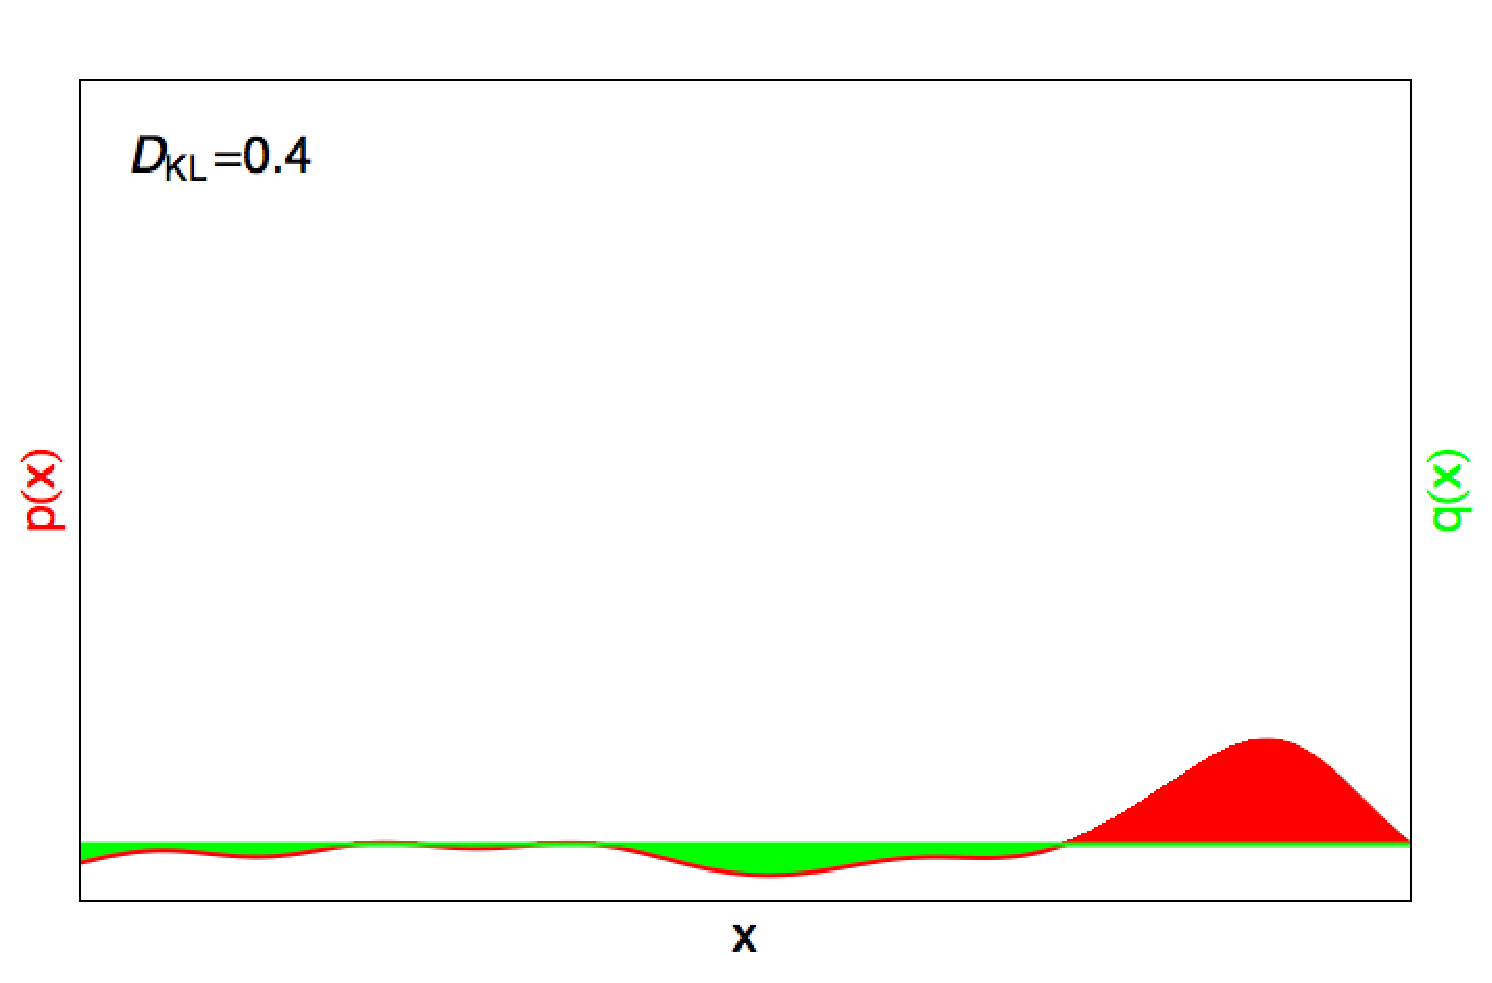
\includegraphics[width=2.4in]{Sanderson_Robyn_fig2_b.eps}   
%\end{tabular} 
%  \caption{}
%   \label{RES:fig2} 
%\end{center}
%\end{figure}
 
 \section{Construction of a mock Milky Way stellar halo}
 
 To test how well the KLD can recover the potential when used as a goodness-of-fit criterion, we constructed a mock Milky Way stellar halo by simulating the disruption of a set of satellite galaxies consistent with current expectations from observations and cosmological simulations. 
 
Satellite galaxy luminosities were drawn from the measured luminosity function of Milky Way satellites given by \cite[Koposov \etal\ (2008)]{Koposov2008} and placed on the fundamental plane of \cite[Tollerud \etal\ (2011)]{Tollerud2011}. We considered only the RGB stars of each satellite, calculating the number per satellite by assuming a stellar mass-to-light ratio of 2 and 1 RGB star per 40 $M_{\odot}$ of stellar mass (\cite[Marigo \etal, 2008]{Marigo2008}; \cite[Helmi \etal, 2011]{Helmi2011}). We limited the mass range of the satellites on the low end by requiring a minimum of 20 RGB stars per satellite and on the high end by setting a maximum velocity dispersion of $\sigma = 20$ km \unit{s}{-1}. Satellites were represented by Plummer spheres in equilibrium at zero tide, with scale radii and masses derived from the fundamental plane parameters using the relations in \cite[Wolf \etal (2010)]{Wolf2010}.

Apocenter radii of satellite center-of-mass orbits were chosen for consistency with the observed radial density distribution of the stellar halo, $\rho \propto r^{-3.5}$ \cite[(Helmi \& de Zeeuw, 2002)]{Helmi2002}. More massive satellites had a higher probability of being placed on an orbit with smaller apocenter, to mimic the effect of dynamical friction. Orbits were distributed uniformly in angle; eccentricities were drawn from the distribution found by \cite[Wetzel \etal\ (2011)]{Wetzel2011} for infalling satellite galaxies in cosmological simulations of Milky-Way-mass halos.  The stars in each satellite were integrated as test particles in the static isochrone potential representing the Galaxy for a random (real) number of orbital periods with a lower limit of 5 orbits and an upper limit of 13.6 Gyr total orbital time. 
 
The number of satellites in the mock halo was chosen so the number of thin streams ($M_* < 10^5 M_\odot$) in which more than 20 RGB stars had acceptable Gaia errors was consistent with current estimates from semi-analytic modeling of the Aquarius simulations (\cite[Helmi \etal, 2011]{Helmi2011}, \cite[Helmi, priv. comm.]{Helmi2013}). This resulted in a stellar halo comprised of 153 streams with more than 20 stars in Gaia range, of which 110 were thin. The positions and velocities of the stars were convolved with the Gaia error model representing its projected performance (\cite[de Bruijne, 2012]{DeBruijne2012}) for KIII giant stars with $M_V = 1$.

\section{Selecting stars without stream membership information}
The KLD is insensitive to which stars belong to a particular clump, and so does not require information about membership of stars in streams. However, the method works best when the action-space clumps are not significantly overlapped. We select stars to use in the fit by guessing a simple form for the energy, 
\begin{equation}
\sub{E}{trial} = \half \mathbf{v}\cdot\mathbf{v} - (220 \textrm{km }\unit{s}{-1})^2 \ln r - \phi_0,
\end{equation}
and viewing the halo stars in the space $(L_z, \sub{E}{trial})$ (Figure \ref{RES:fig3}, left panel). The constant $\phi_0$ is chosen so that all $\sub{E}{trial}<0$. We select all stars for which $\sub{E}{trial}>\sub{E}{cut}$, and set $\sub{E}{cut}$ to select the part of the distribution that looks clumpy to the eye. After trying several different values, we chose $\sub{E}{cut} = -0.64 \unit{ kpc}{2}\unit{ Myr}{-2}$ (blue dashed line in left panel of Figure \ref{RES:fig3}). The selected sample contains 195166 stars in 39 streams, with a bias towards more distant streams (Figure \ref{RES:fig3}, right panel). Although the observational errors blur the streams in action space, individual streams still form clumps (Figure \ref{RES:fig4}).

\begin{figure}
\begin{center}
\begin{tabular}{cc}
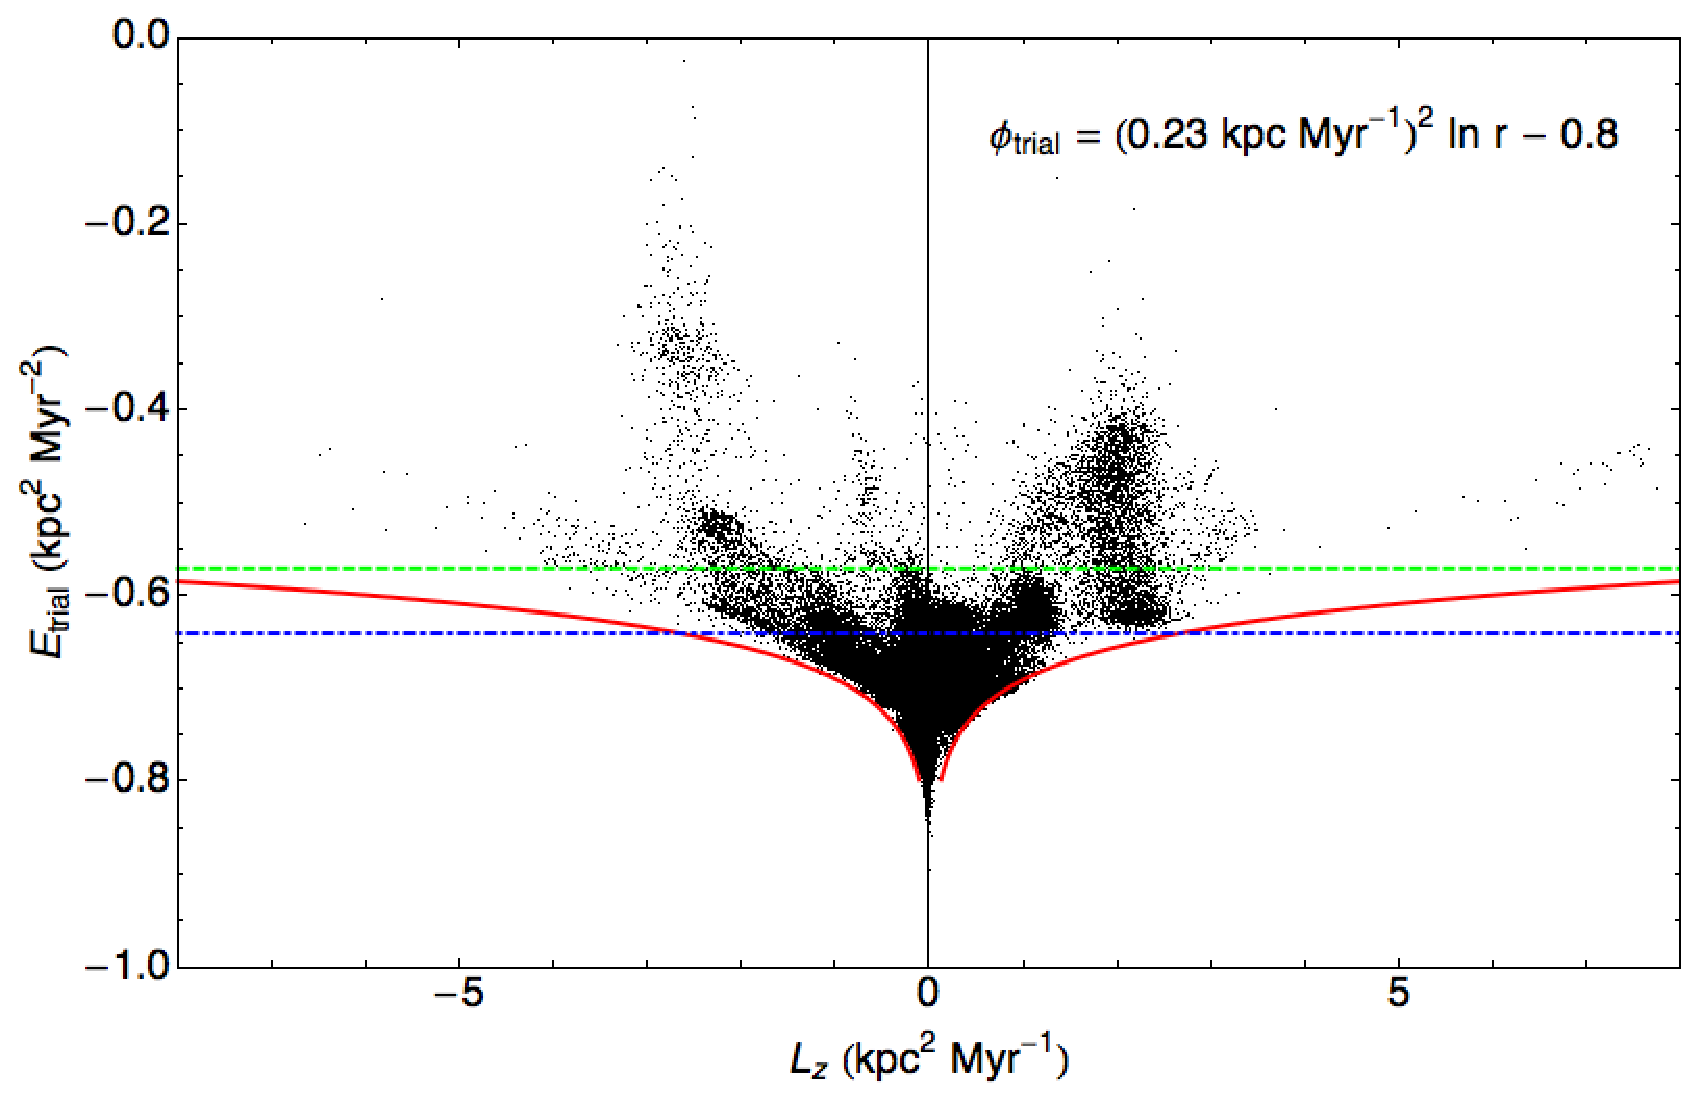
\includegraphics[width=2.4in]{Sanderson_Robyn_fig3a.ps} & 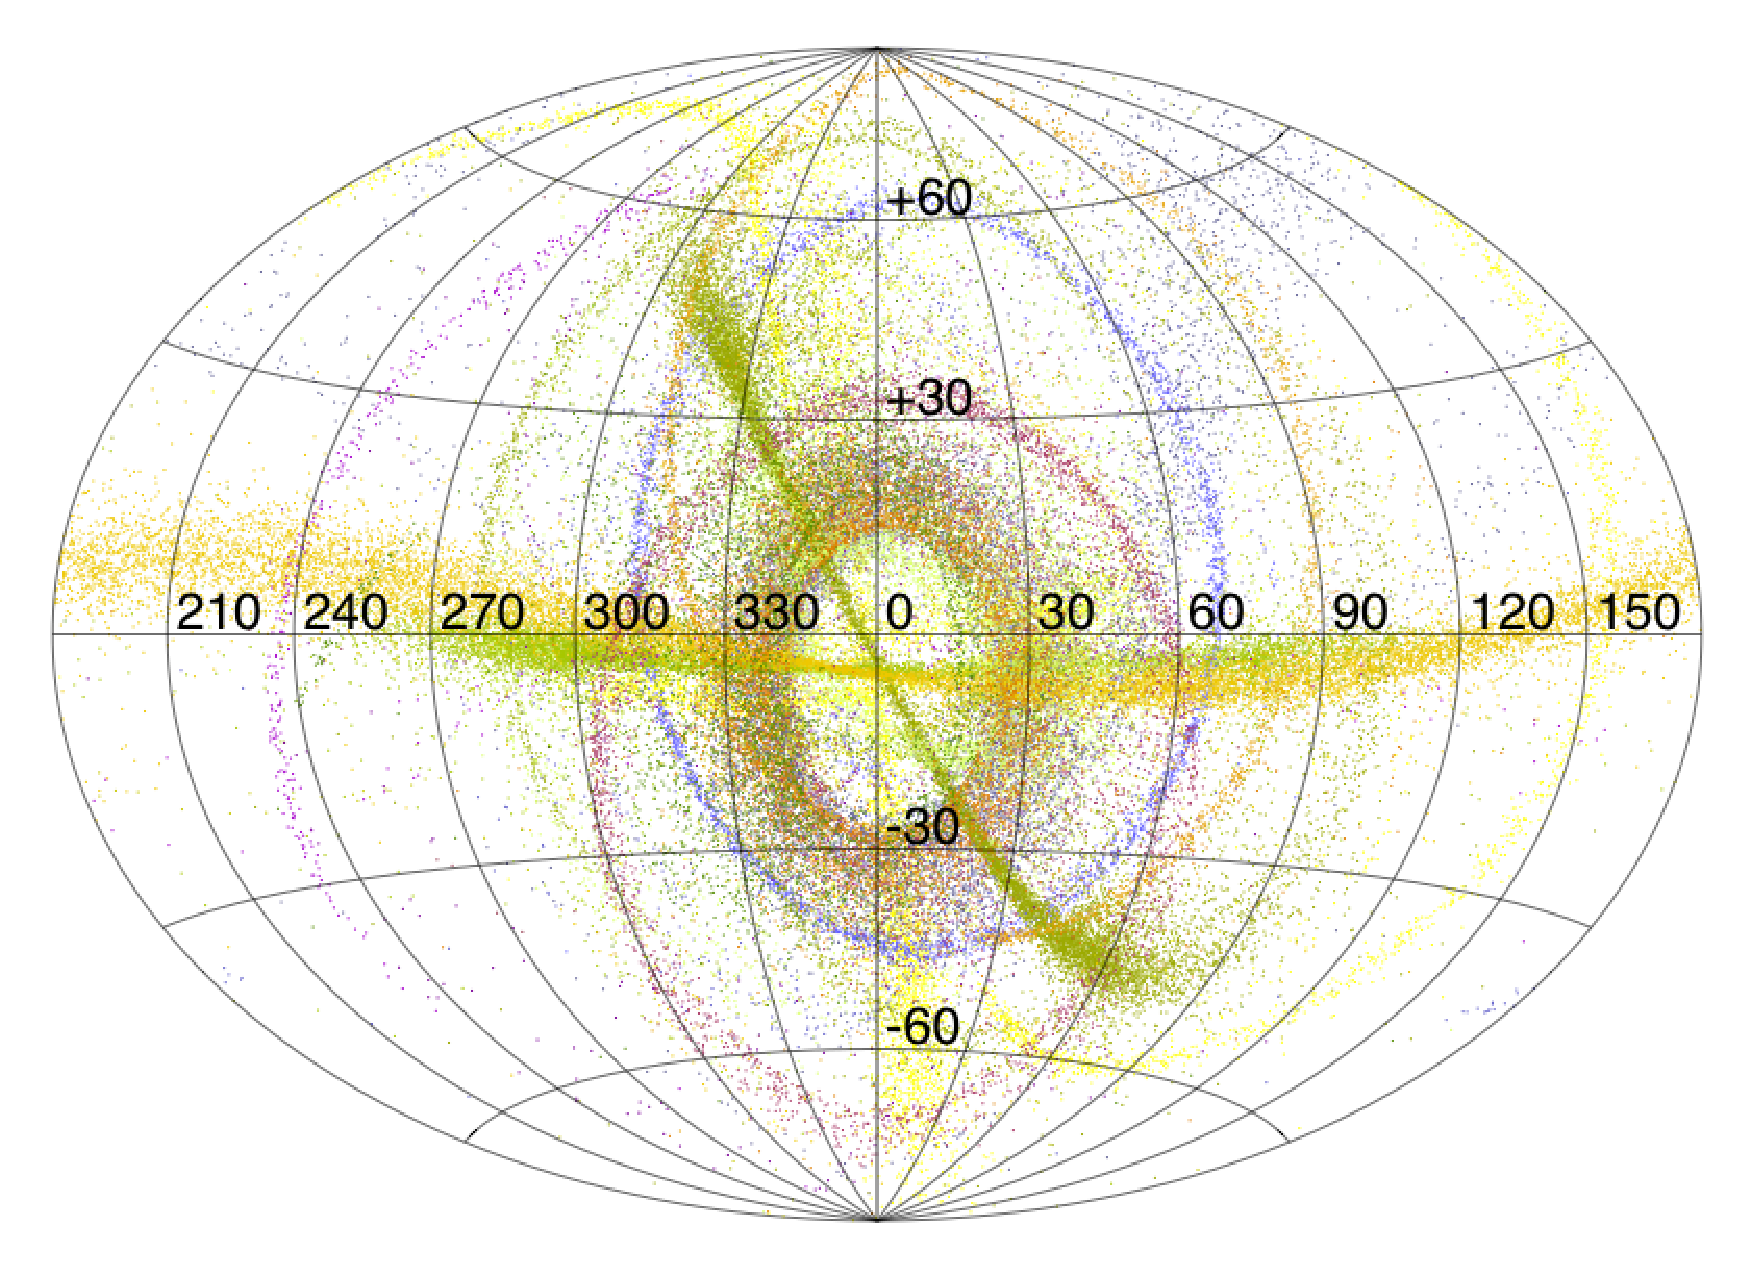
\includegraphics[width=2.4in]{Sanderson_Robyn_fig3b.ps} 
\end{tabular}
\caption{Left: Approximate energy-angular momentum space used to select stars for potential fitting. All stars above the blue line are used for the fit. Right: Selected stars in Galactic coordinates (different colors indicate different progenitors).}
\label{RES:fig3}
\end{center}
\end{figure}

\begin{figure}
\begin{center}
\begin{tabular}{cc}
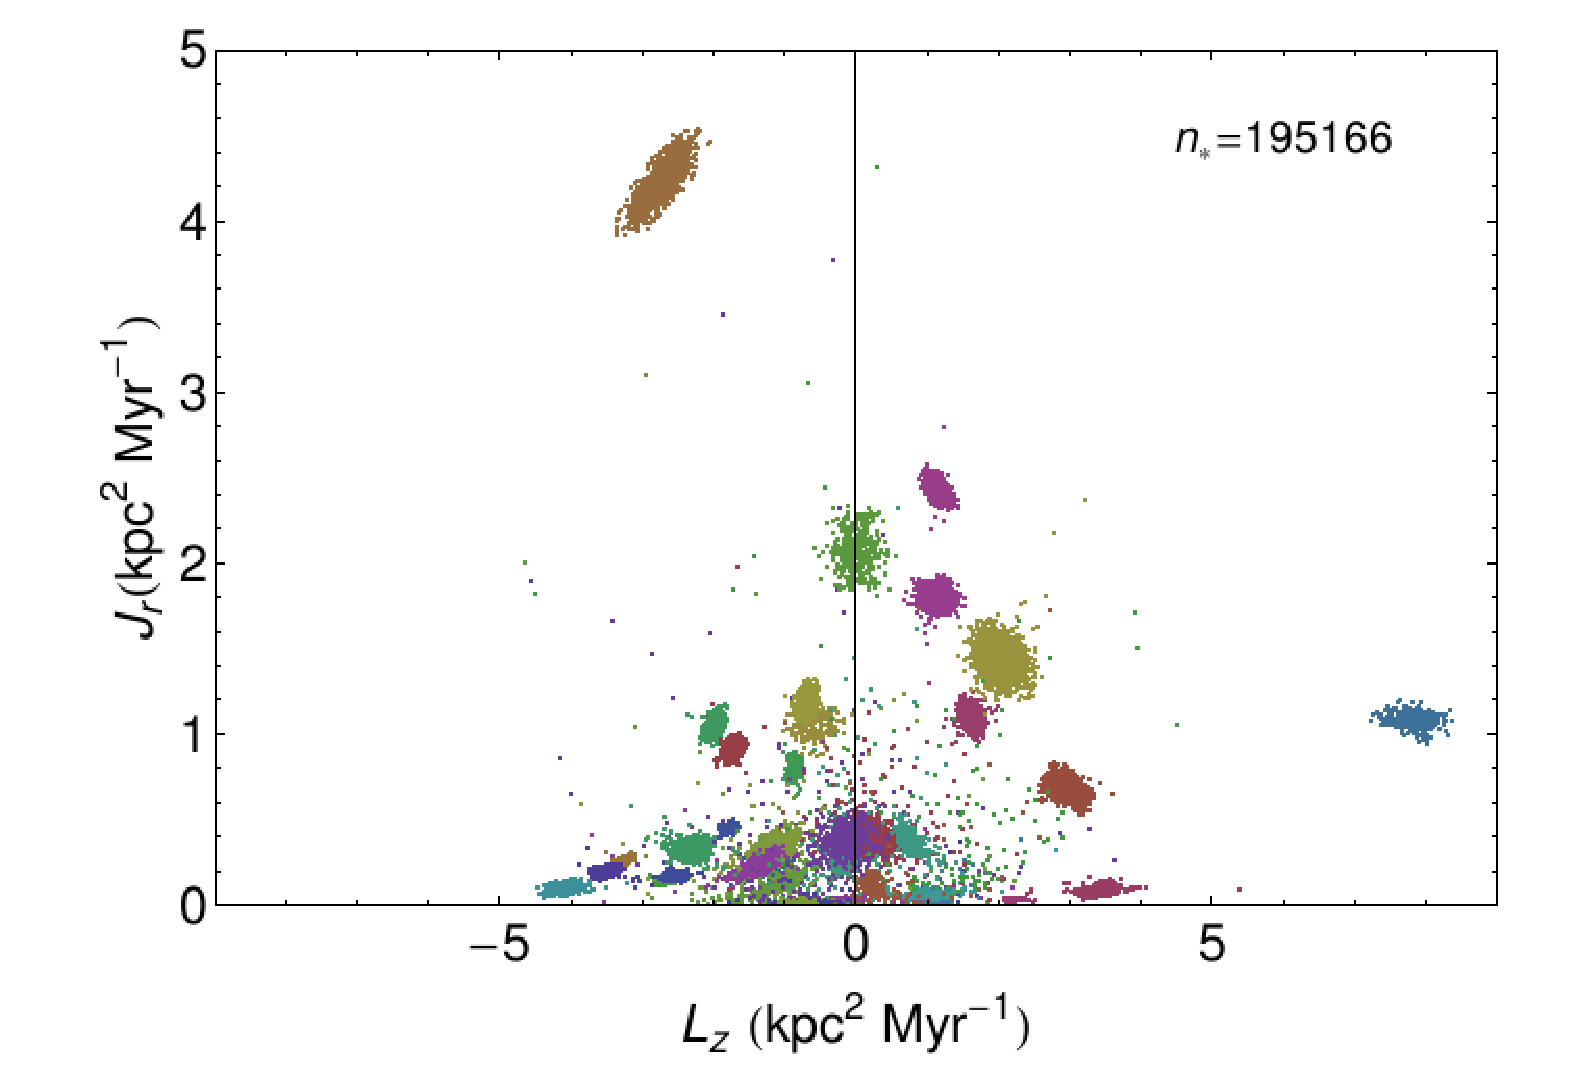
\includegraphics[width=2.4in]{Sanderson_Robyn_fig4a.ps} & 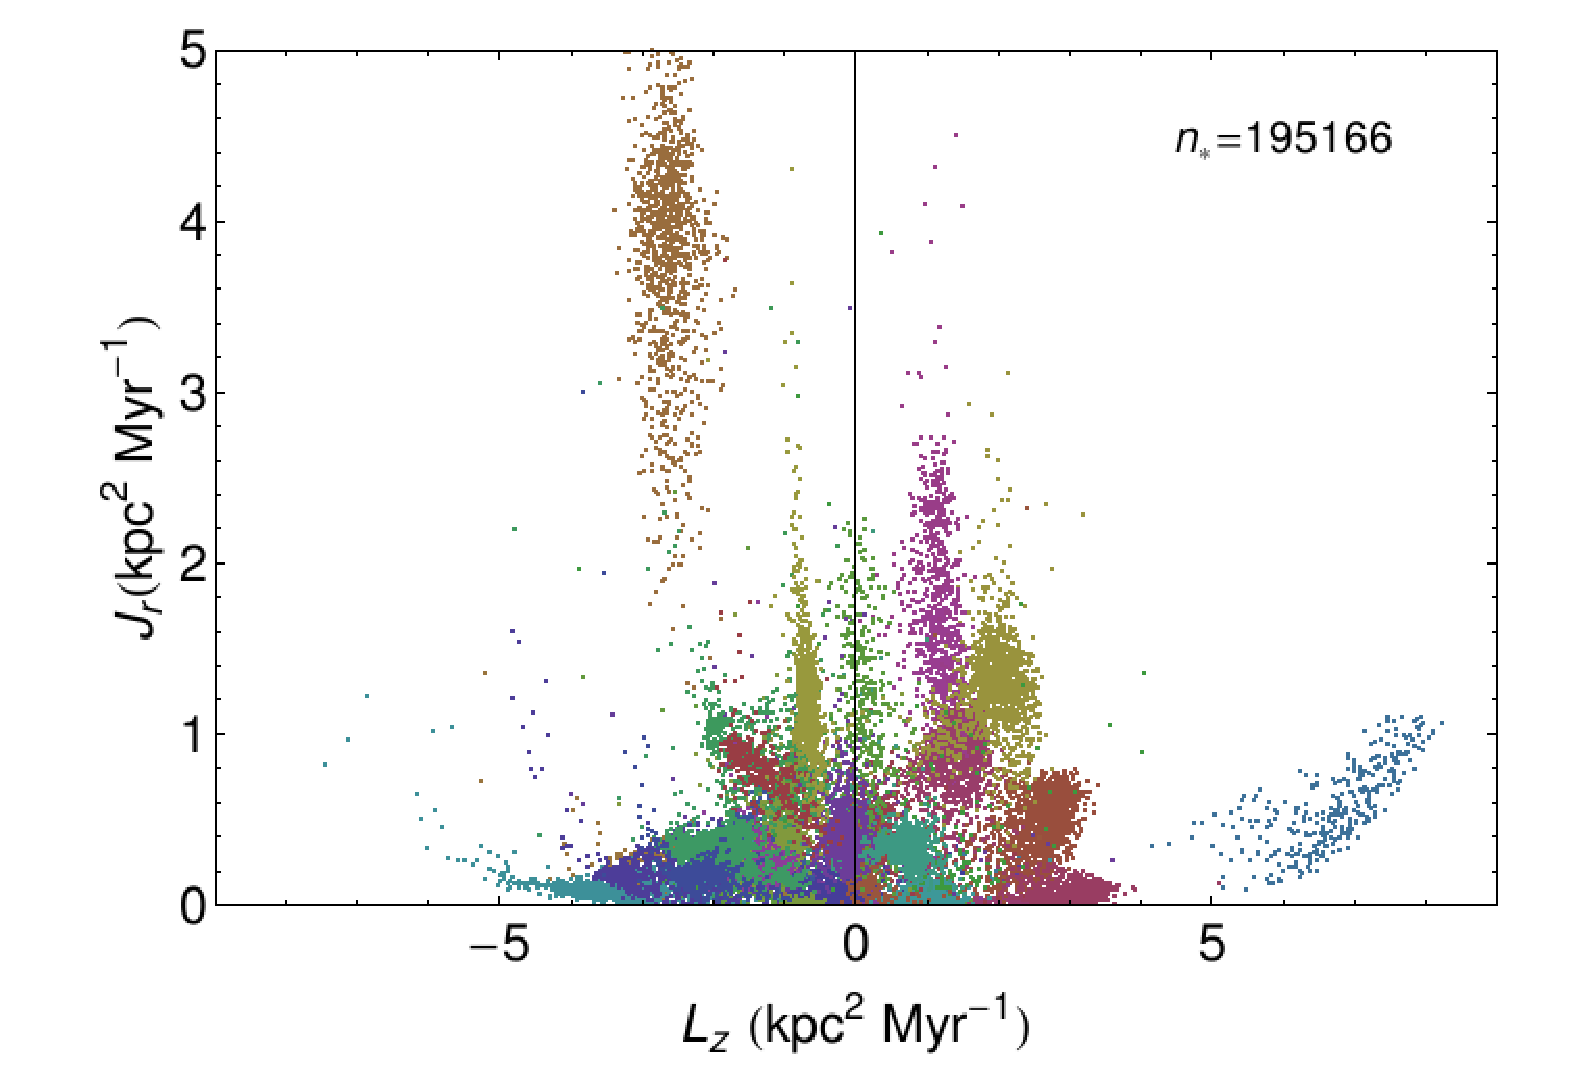
\includegraphics[width=2.4in]{Sanderson_Robyn_fig4b.ps}
\end{tabular}
\caption{Selected stars in the projected action space $(L_z,J_r)$ for the correct potential parameters, without (left) and with (right) Gaia errors. Different colors indicate different progenitors. $n_*$ is the number of stars in the sample.}
\label{RES:fig4}
\end{center}
\end{figure}

\section{Fitting potential parameters using the KLD in two steps}
To identify the best-fit potential, we tiled the two-dimensional parameter space with a regular grid of points spaced by 0.05-dex in $\log_{10} (M/M_\odot)$ and $\log_{10} (b/\textrm{kpc})$. For each combination $\mathbf{a} = (M,b)$ we calculate $(J_r, L, L_z)$ for each star in the selected sample to produce a three-dimensional distribution of actions $f(\mathbf{J}|\mathbf{a})$, discarding $\mathbf{a}$ if more than 1 percent of the stellar orbits are unbound. Then we randomize the $L$ and $L_z$ values of the stars, which do not depend on $\mathbf{a}$, to produce a comparison distribution $f(\sub{\mathbf{J}}{shuf}|\mathbf{a})$. Randomization guarantees that the $\sub{\mathbf{J}}{shuf}$ are less clustered than the $\mathbf{J}$. We use a density estimator to calculate the Kullback-Liebler distance between these two distributions, $\sub{D^{(1)}}{KL} = \sub{D}{KL}\left[ f(\mathbf{J}|\mathbf{a}) || f(\sub{\mathbf{J}}{shuf}|\mathbf{a})\right]$. The point $\mathbf{a}_0$ with largest $\sub{D^{(1)}}{KL}$ is the best-fit potential.

Once the best-fit is identified we use a second step to determine how well the parameters are recovered. In this step we calculate the KLD between the action distribution at the best-fit parameters, $f(\mathbf{J}|\mathbf{a}_0)$, and the action distribution $f(\mathbf{J}|\mathbf{a})$ for each point in the parameter grid: $\sub{D^{(2)}}{KL} = \sub{D}{KL}\left[ f(\mathbf{J}|\mathbf{a}_0) || f(\mathbf{J}|\mathbf{a})\right]$. Since the distribution is most clustered at $\mathbf{a}_0$, $\sub{D^{(2)}}{KL}$ will be zero at $\mathbf{a}_0$ and increase away from this minimum. \cite[Kupperman (1957)]{kupperman1957} relates  $\sub{D^{(2)}}{KL}$ to the $\chi^2$ distribution for a system with $n_0$ data points (stars) and $m_0$ degrees of freedom:
\begin{equation}
2 n_0 \sub{D}{KL}\left[ f(\mathbf{J}|\mathbf{a}_0) || f(\mathbf{J}|\mathbf{a})\right] \to \chi^2(m_0 \textrm{ DOF})
\end{equation}
as $n_0 \to \infty$. In this way we can assign a $\chi^2$ value to each $\mathbf{a}$.

\section{Results}
For the stars selected from our mock halo, the best-fit potential parameters identified by our method in the first step described above are within 1 parameter grid point of the input values; that is, within $\sim$0.05 dex (Figure \ref{RES:fig5}, left panel). After step 2, we see that the $1\sigma$ confidence interval, which is too small to be adequately sampled at this grid spacing, is roughly $\pm 0.1$ dex in both parameters, and the input values are well within the $2\sigma$ contour (Figure \ref{RES:fig5}, right panel). 

\begin{figure}
\begin{center}
\begin{tabular}{cc}
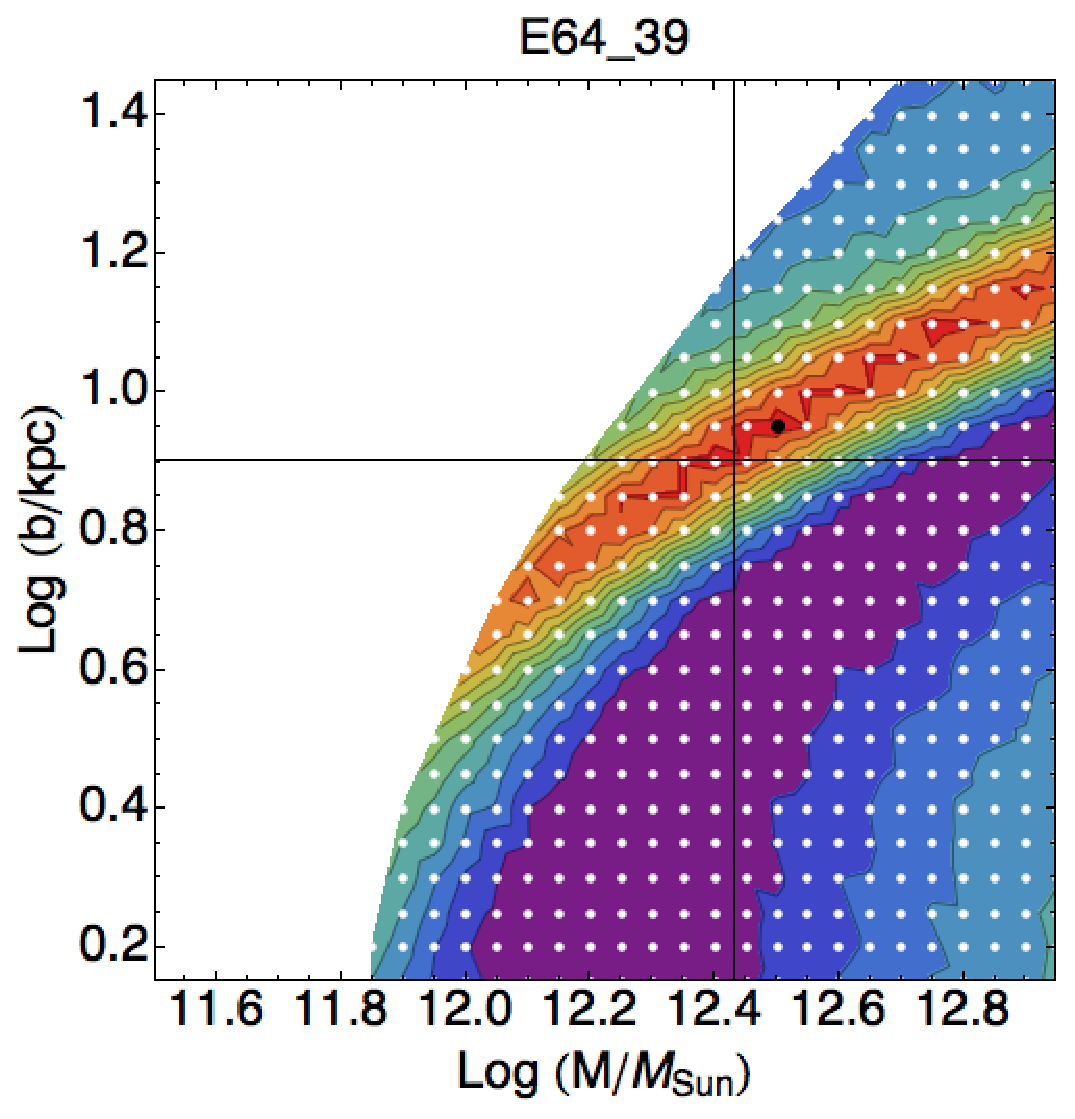
\includegraphics[width=2.4in]{Sanderson_Robyn_fig5a.eps} & 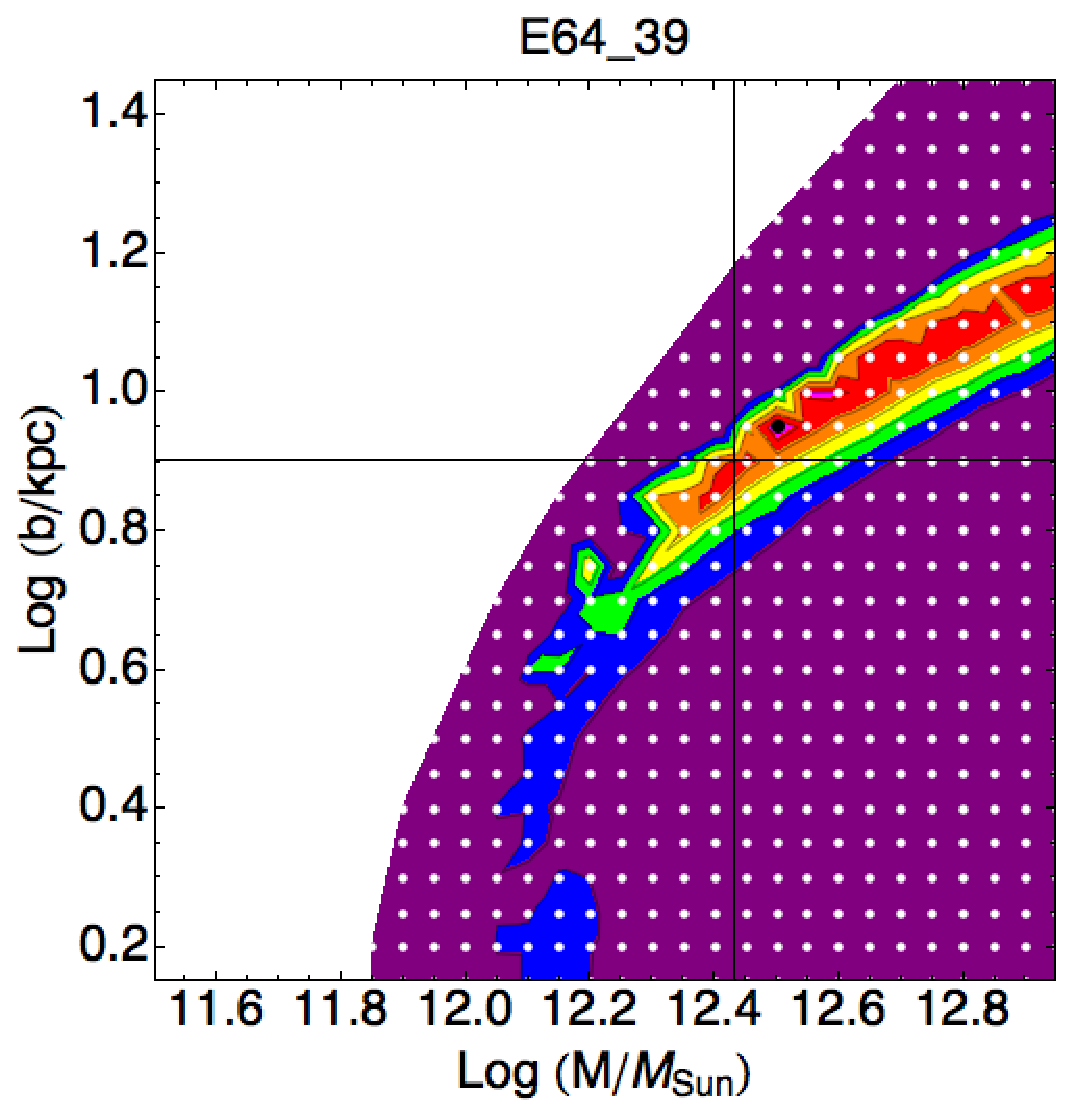
\includegraphics[width=2.4in]{Sanderson_Robyn_fig5b.eps}
\end{tabular}
\caption{Contour plots of $\sub{D^{(1)}}{KL}$, used to identify the best-fit potential (left), and $\chi^2 \propto \sub{D^{(2)}}{KL}$, used to determine the confidence intervals on the parameters (right). In both plots, the black dot identifies the best-fit potential parameters, the black lines cross at the input values, and the white dots show the parameter grid. In the white region more than 1\% of star orbits are unbound. The contours in the left-hand plot are evenly spaced in $\sub{D^{(1)}}{KL}$; the contours of the right-hand plot show $\chi^2/\textrm{DOF}<\{1,2,3,4,5,6\}$ for the colors $\{$magenta, red, orange, yellow, green, blue$\}$. }
\label{RES:fig5}
\end{center}
\end{figure}

We tested how the ability to recover the true potential was affected by the number of streams by building up a random subset of streams from $\sub{N}{str}=1$ to $\sub{N}{str}=39$ (the full sample). The recovery generally improves as the number of streams increases (Figure \ref{RES:fig6}). For $\sub{N}{str}\lesssim 20$, the process is still sensitive to the particular streams that make up the sample, and adding another stream can substantially change the result. Above this threshold adding one more stream tends to affect the best-fit values much less and by this point the chi-squared contours are nearly as small as in the full sample.

\begin{figure}
\begin{center}
\begin{tabular}{ccc}
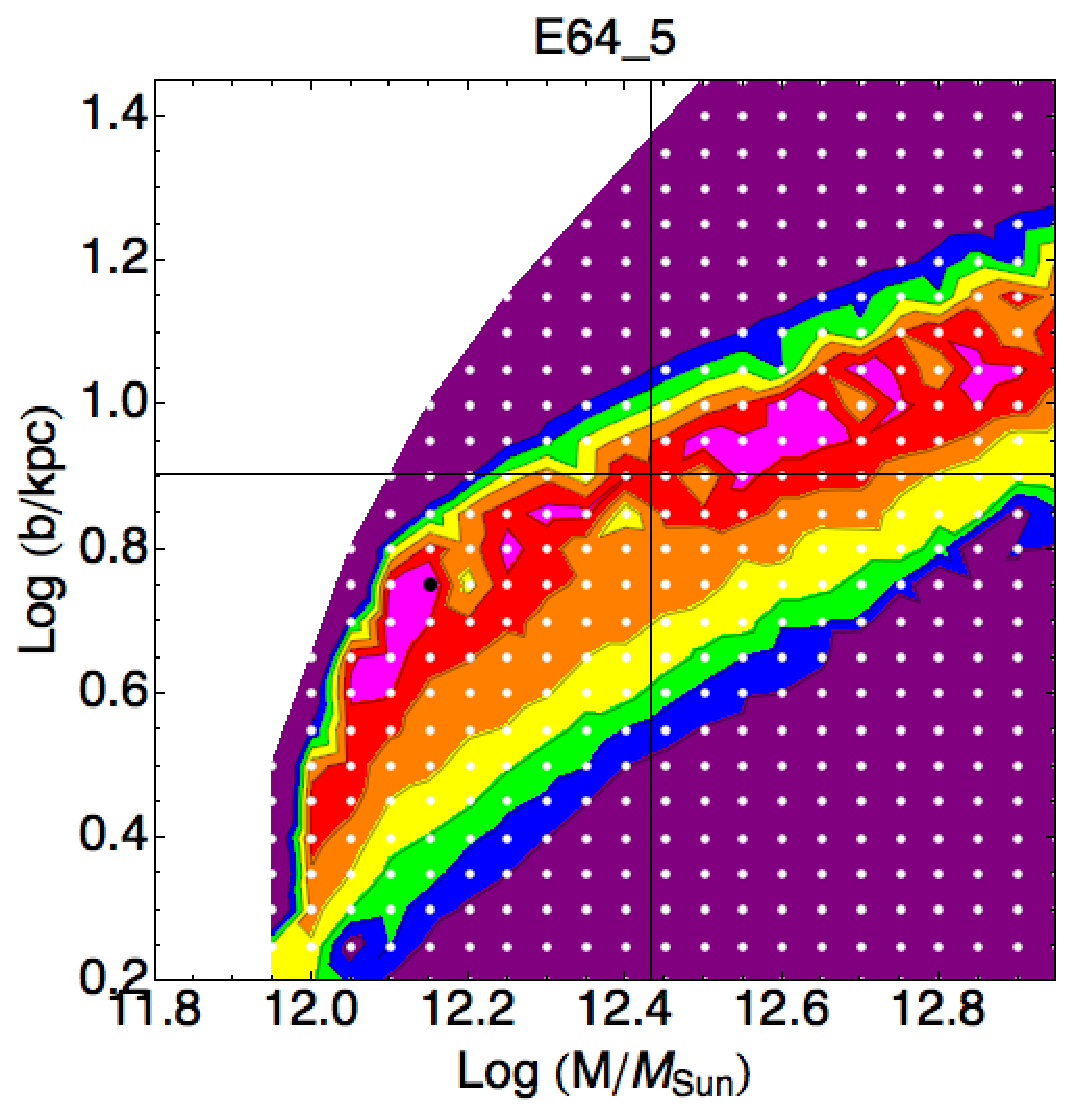
\includegraphics[width=1.6in]{Sanderson_Robyn_fig6a.eps} & 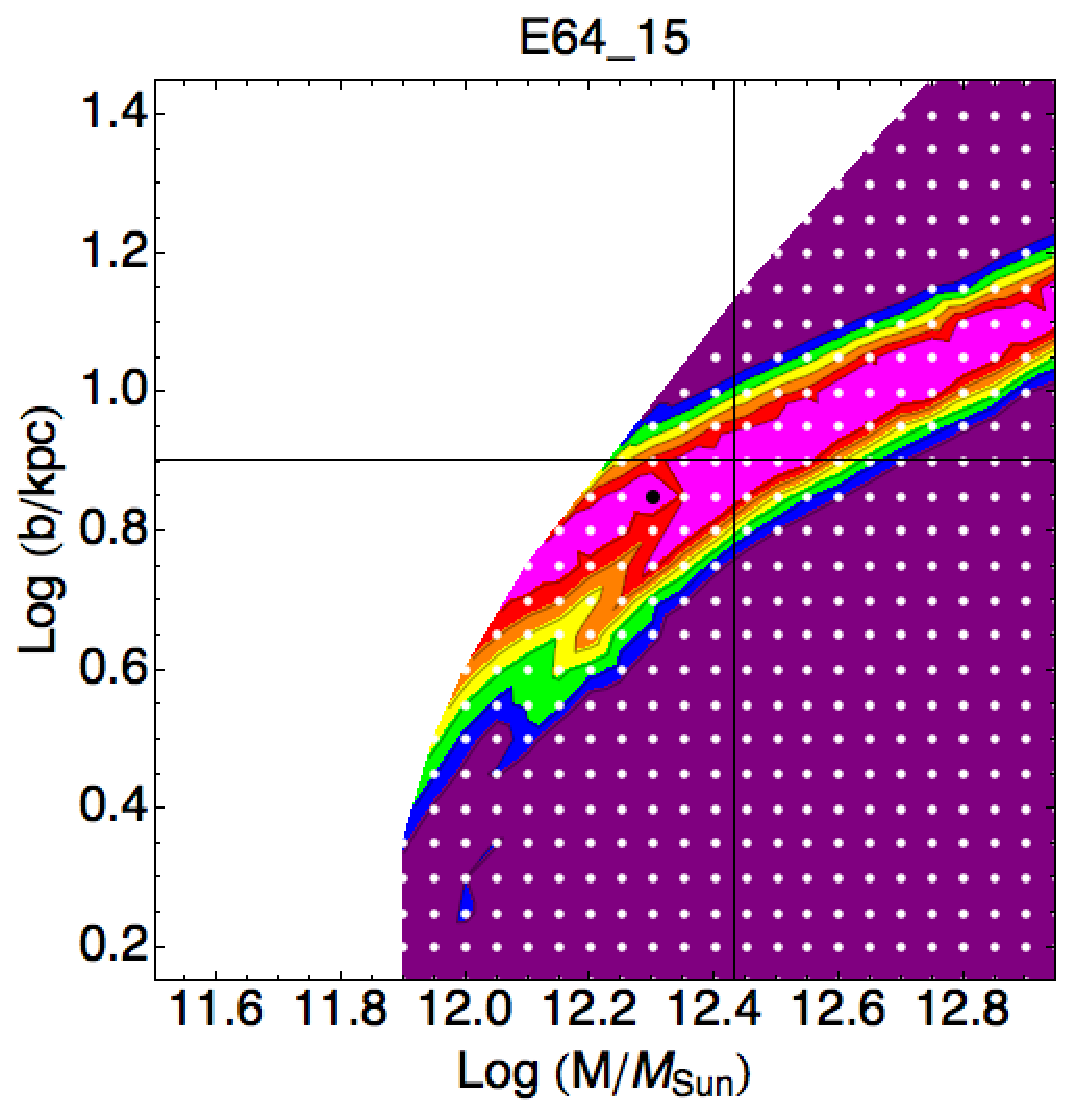
\includegraphics[width=1.6in]{Sanderson_Robyn_fig6b.eps} & 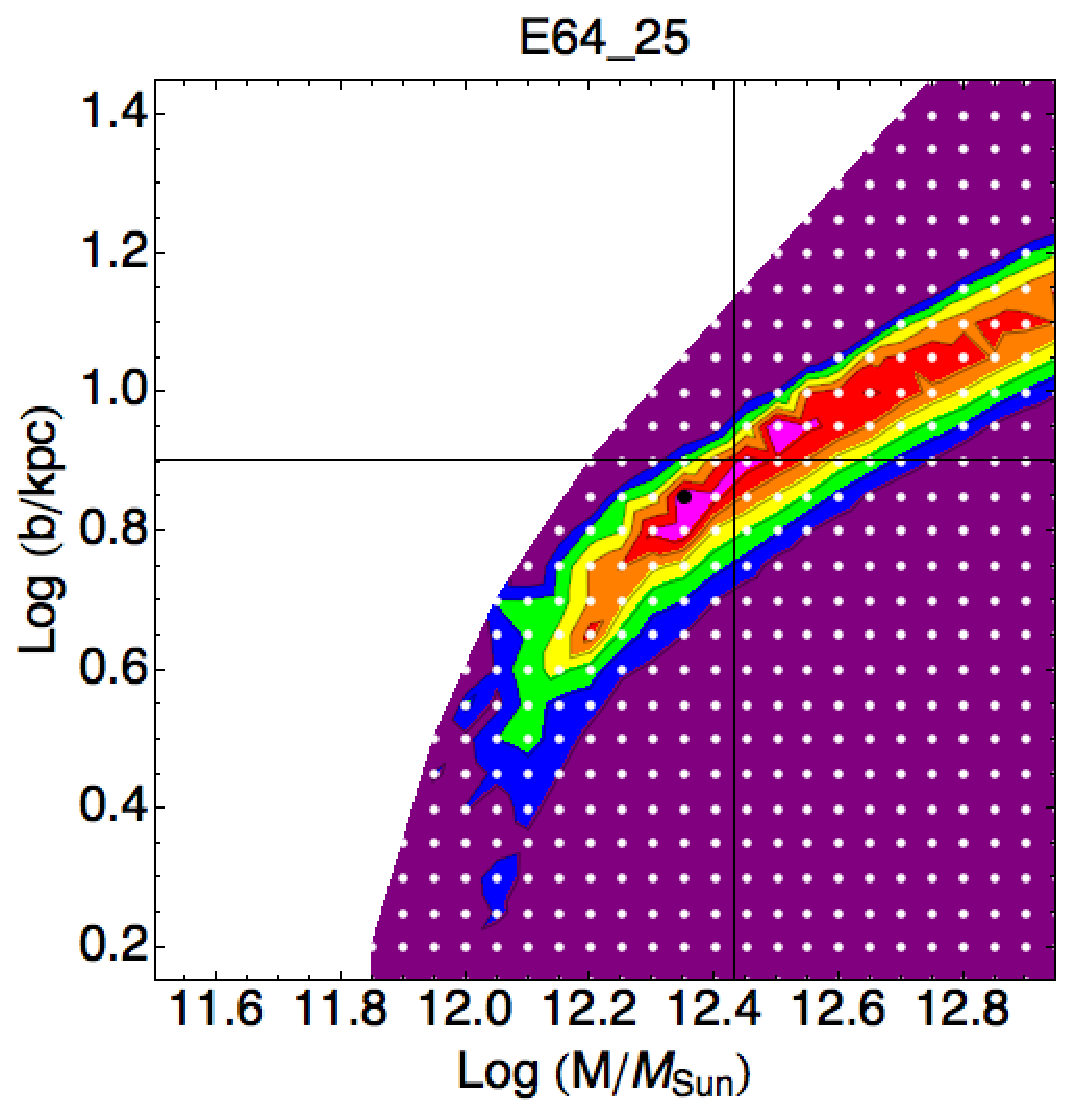
\includegraphics[width=1.6in]{Sanderson_Robyn_fig6c.eps}
\end{tabular}
\caption{Contour plots of $\chi^2/\textrm{DOF}$, as in the right panel of Figure \ref{RES:fig5}, but for different numbers of streams.}
\label{RES:fig6}
\end{center}
\end{figure}

\section{Conclusions \& future work}
Maximizing the clustering of tidal streams in action space, measured by the KLD, can recover the true potential given the errors and number of streams predicted for Gaia. This technique does not require stream membership information, and returns uncertainties as well as best-fit values for the potential parameters. In our tests about 20 streams are needed to overcome variability from individual streams; using all the observed streams in our mock halo results in $1\sigma$ confidence intervals of about 0.1 dex in each parameter.

In the future we will extend this work to more realistic potentials (axisymmetric, triaxial, and/or time-dependent). This fitting algorithm also provides a framework for comparing the ability of different models to fit the potential if the Bayesian evidence can be calculated. Finally, including more realistic stellar populations in the mock halo will reveal the full impact of Gaia spectroscopic follow-up missions like WEAVE and 4MOST to constrain the potential. 


\begin{thebibliography}{}

\bibitem[de Bruijne, 2012]{DeBruijne2012}{de Bruijne, J. H. J.} 2012, arXiv:1201.3238
\bibitem[Koposov \etal\ (2008)]{Koposov2008}{Koposov, S., Belokurov, V., Evans, N. W., Hewett, P. C., Irwin, M. J., Gilmore, G., Zucker, D. B., Rix, H.-W., Fellhauer, M., Bell, E. F., \& Glushkova, E. V.} 2008, \textit{ApJ}, 686, 279
\bibitem[Kupperman (1957)]{kupperman1957}{Kupperman, J.} 1957, Ph.D. Thesis, Georgetown University
\bibitem[Helmi \etal, 2011]{Helmi2011}{Helmi, A., Cooper, A. P., White, S. D. M.,  Cole, S., Frenk, C. S., \& Navarro, J. F.} 2011, \textit{ApJ}, 733, L7
\bibitem[Helmi, priv. comm.]{Helmi2013}{Helmi, A.} 2013, priv. comm.
\bibitem[Marigo \etal, 2008]{Marigo2008}{Marigo, P., Girardi, L., Bressan, A.,  Groenewegen, M. A. T., Silva, L., \& Granato, G. L.} 2008, \textit{A\&A}, 482, 883
\bibitem[Tollerud \etal\ (2011)]{Tollerud2011}{Tollerud, E. J., Bullock, J. S., Graves, G. J., \& Wolf, J.} 2011, \textit{ApJ}, 726, 108
\bibitem[Wetzel \etal\ (2011)]{Wetzel2011}{Wetzel, A. R.} 2011, \textit{MNRAS}, 412, 49
\bibitem[Wolf \etal (2010)]{Wolf2010}{{Wolf}, J. , {Martinez}, G.~D. , {Bullock}, J.~S. , {Kaplinghat}, M. , {Geha}, M. , {Mu{\~n}oz}, R.~R. , {Simon}, J.~D. , \& {Avedo}, F.~F.}

%\bibitem[Amari \etal\ (1995)]{Amari_etal95}
%{Amari, S., Hoppe, P., Zinner, E., \& Lewis R.S.} 1995,
%\textit{Meteoritics}, 30, 490 
%
%\bibitem[Anders \& Zinner (1993)]{AndersZinner93}
%{Anders, E., \& Zinner, E.} 1993, 
%\textit{Meteoritics}, 28, 490
%
%\bibitem[Bernatowicz et al. (2003)]{Bernatowicz_etal03}
%{Bernatowicz, T.J., Messenger, S., Pravdivtseva, O., Swan, P., \& Walker, R.M.} 2003, 
%\textit{Geochim. Cosmochim. Acta}, 67, 4679
%
%\bibitem[Busso et al. (1999)]{Busso_etal99}
%{Busso, M., Gallino, R., \& Wasserburg, G.J.} 1999, 
%\textit{ARAA}, 37, 239
%
%\bibitem[Croat, Stadermann \& Bernatowicz (2005)]{Croat_etal05}
%{Croat, T.K., Stadermann, F.J., \& Bernatowicz, T.J.} 2005, 
%\textit{ApJ}, 631, 976
%
%\bibitem[Draine (2003)]{Draine03}
%{Draine, B.T.} 2003,
%\textit{ARAA}, 41, 241
%
%\bibitem[Hoppe \& Zinner (2000)]{HoppeZinner00}
%{Hoppe, P., \& Zinner, E.} 2000, 
%\textit{J. Geophys. Res.}, A105, 10371
%
%\bibitem[Hoppe, Ott \& Lugmair (2004)]{Hoppe_etal04}
%{Hoppe, P., Ott, U., \& Lugmair, G.W.} 2004, 
%\textit{New Astron. Revs}, 48, 171
%
%\bibitem[Lodders \& Fegley (1998)]{LoddersFegley98}
%{Lodders, K., \& Fegley, B.} 1998, 
%\textit{Meteorit. Planet. Sci.}, 33, 871
%
%\bibitem[Meyer, Clayton \& The (2000)]{Meyer_etal00}
%{Meyer, B.S., Clayton, D.D., \& The, L.-S.} 2000, 
%\textit{ApJ} (Letters), 540, L49
%
%\bibitem[Nittler (2003)]{Nittler03}
%{Nittler, L.R.} 2003, 
%\textit{Earth Planet. Sci. Lett.}, 209, 259
%
%\bibitem[Nittler et al. (1997)]{Nittler_etal97}
%{Nittler, L.R., Alexander, C.M.O'D., Gao, X., Walker, R.M., \& Zinner, E.} 1997,
%\textit{ApJ}, 483, 475
%
%\bibitem[Ott (1993)]{Ott93}
%{Ott, U.} 1993, 
%\textit{Nature}, 364, 25
%
%\bibitem[Ott (2002)]{Ott02}
%{Ott, U.} 2002,
%\textit{New Astron. Revs} 46, 513
%
%\bibitem[Ott et al. (2005)]{Ott_etal05}
%{Ott, U., Altmaier, M., Herpers, U., Kuhnhenn, J., Merchel, S., 
%Michel, R., \& Mohapatra, R.K.} 2005, 
%\textit{Meteorit. Planet. Sci.}, 40, 1635
%
%\bibitem[Yin, Lee \& Ott (2006)]{Yin_etal06}
%{Yin, Q.-Z., Lee, C.-T. A., \& Ott, U.} 2006, 
% \textit{ApJ}, 647, 676
%
%\bibitem[Zinner (1998)]{Zinner98}
%{Zinner, E.} 1998,
% \textit{Ann. Rev. Earth Planet. Sci.}, 26, 147
%
%\bibitem[Zinner (2004)]{Zinner04}
%{Zinner, E.} 2004, in: K.K. Turekian, H.D. Holland \& A.M. Davis (eds.), 
 %\textit{Treatise in Geochemistry 1} (Oxford and San Diego: Elsevier), p.\,17

\end{thebibliography}

\begin{discussion}

\discuss{Grillmair}{Is your technique sensitive to the length of the tidal streams in the sample?}

\discuss{Answer}{No, we actually discard that information since we consider only the actions and not the angles of the stream stars. This is probably why it takes 20 streams to get a good fit when in principle you could do it with only one.}

\discuss{Zhao}{What happens if there are stars in your sample that don't belong to a stream, but to a smooth background?}
\discuss{Answer}{This will affect the results only if enough stars belong to the smooth background that the stream-clusters are lost in the noise. The KLD can also be maximized by increasing the mass and decreasing the scale radius of the potential without bound, thereby putting all the stars into one big clump deep in the potential. If there is too much smooth background, this asymptotic region starts to get a KLD higher than the local maximum that identifies the best-fit potential. This is why we choose an energy cutoff to select the stars for the fit---if you include all of them, the clumps at low $(J_r,L_z)$ all blend together and produce the same effect.}


\end{discussion}

\end{document}
